\section{Hummus}
% Linke Seite: Rezept
Zutaten:
\begin{itemize}
    \item 1 Dose gekochten Kichererbsen (ca. 800g)
    \item 1-2 El. Tahina (Sesam-Mus)
    \item Salz und Pfeffer
    \item 1/2 Zitrone
    \item (Beilage) Tortillas
    \item (Beilage) Jasmin-Reis
\end{itemize}


\noindent Zubereitung:

\noindent Kichererbsen in Topf füllen und leicht mit Wasser becken. Zugedeckt
etwa 20 Minuten kochen. Wasser abschütten und 2 El. Wasser hinzugeben.
Zitronensaft der 1/2 Zitrone zugeben. Tahina hinzugeben. Alles pürieren. Mit
Salz, Pfeffer, und zusätzlichem Tahina abschmecken.

Mit Reis in Tortillas einrollen und servieren.

% Recht Seite: Bild
\newpage
\mbox{}
\vfill
\begin{center}
    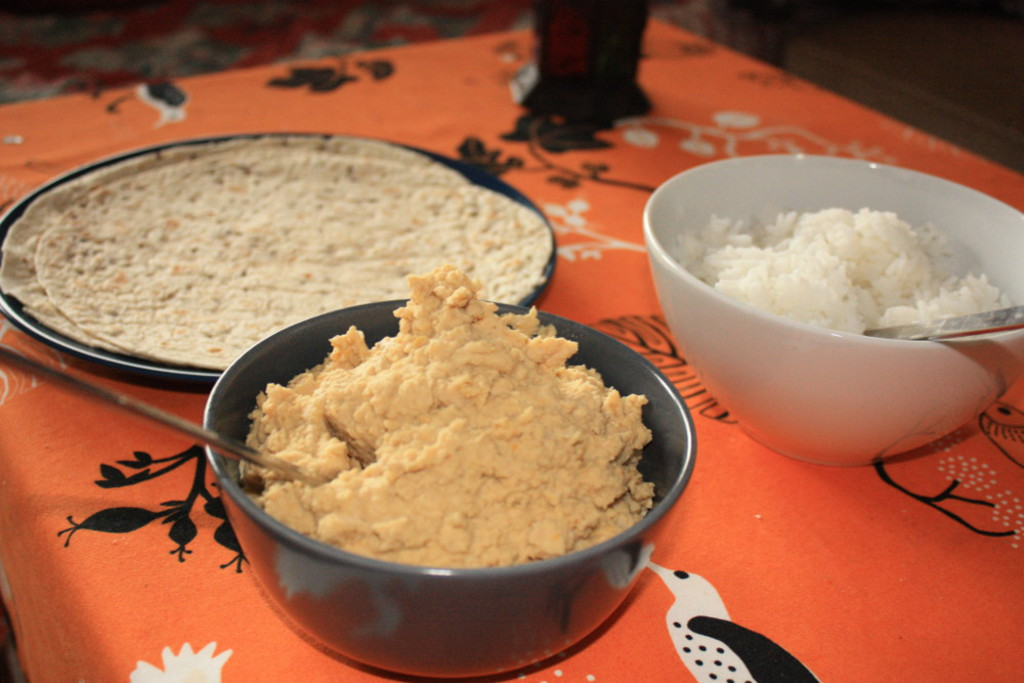
\includegraphics[width=\textwidth]{Hummus/IMG_6096_small.jpg}
\end{center}
\vfill
\mbox{ }
\newpage
